\documentclass[12pt,a4paper]{article}
\usepackage[utf8]{vietnam}
\usepackage{amsmath,amssymb}
\usepackage{tabularx}
\usepackage{tikz}
\usetikzlibrary{calc,angles,quotes,arrows.meta,patterns}
\usepackage{xcolor}
\usepackage{enumitem}
\usepackage{fancyhdr}
\usepackage{graphicx}
\usepackage[top=0.9cm, bottom=0.9cm, left=1.2cm, right=1.2cm]{geometry}
\usepackage[dethi]{ex_test}
\SAOPTN{widthSA=3.2,heightSA=0.62}

\setlength{\headheight}{15pt}
\setlength{\parskip}{0pt}

\pagestyle{fancy}
\fancyhf{}
\rhead{\textit{Môn Toán 9 -- Đề số 08}}
\lhead{\textit{Bộ đề ôn tập Giữa học kì I}}
\cfoot{\thepage}

\begin{document}

% --- KHUNG TIÊU ĐỀ ĐỀ THI ---
\noindent
\begin{tabularx}{\linewidth}{X r}
\textbf{TRƯỜNG THCS: \dotfill} & \textbf{ĐỀ KIỂM TRA ĐỊNH KỲ GIỮA HỌC KỲ I} \\
\textbf{Họ và tên: \dotfill} & \textbf{NĂM HỌC 2026 -- 2027} \\
\textbf{Lớp: \dotfill \quad SBD: \dotfill} & \textbf{Môn: TOÁN 9} \\
\hline
\end{tabularx}
\vspace{2mm}

\begin{center}
  \textbf{\large ĐỀ ÔN TẬP GIỮA HỌC KỲ I -- ĐỀ SỐ 08}\\
  \textit{Thời gian làm bài: 90 phút (Không kể thời gian phát đề)}
\end{center}
\vspace{1mm}

% --- PHẦN I ---
\noindent\textbf{\large PHẦN I. CÂU TRẮC NGHIỆM NHIỀU PHƯƠNG ÁN LỰA CHỌN (3,0 điểm)}

\textit{Thí sinh trả lời từ câu 1 đến câu 12. Mỗi câu hỏi thí sinh chỉ chọn một phương án duy nhất.}

\vspace{1mm}
\begin{ex}
Căn bậc hai của $\frac{4}{9}$ là:
\choice
{$\frac{2}{3}$}
{$-\frac{2}{3}$}
{\True $\pm \frac{2}{3}$}
{$\frac{16}{81}$}
\end{ex}

\begin{ex}
Tìm điều kiện để biểu thức $\frac{1}{\sqrt{3 - x}}$ có nghĩa:
\choice
{\True $x < 3$}
{$x \le 3$}
{$x \ge 3$}
{$x > 3$}
\end{ex}

\begin{ex}
Biểu thức $A = \sqrt{2x^2 + 1}$ xác định với:
\choice
{$x \neq -\frac{1}{2}$}
{\True Mọi $x \in \mathbb{R}$}
{$x \ge -\frac{1}{2}$}
{$x \ge \pm \frac{1}{2}$}
\end{ex}

\begin{ex}
Hệ phương trình nào dưới đây là hệ hai phương trình bậc nhất hai ẩn?
\choice
{$\begin{cases} x + y = 1 \\ y + z = -3 \end{cases}$}
{$\begin{cases} 2x + y = 2 \\ 3x - y^2 = -1 \end{cases}$}
{$\begin{cases} 2x^2 - y = 0 \\ x + y = 0 \end{cases}$}
{\True $\begin{cases} -x + 2y = 1 \\ y = 1 \end{cases}$}
\end{ex}

\begin{ex}
Điều kiện xác định của phương trình $\frac{1}{x + 2} = \frac{1}{x - 1} + 2$ là:
\choice
{$x \neq 1; x \neq -3$}
{\True $x \neq -2; x \neq 1$}
{$x \neq -3; x \neq -2$}
{$x \neq 2; x \neq -1$}
\end{ex}

\begin{ex}
Phát biểu "$a$ không lớn hơn $b$" được biểu diễn bằng bất đẳng thức nào dưới đây?
\choice
{$a < b$}
{\True $a \le b$}
{$a \ge b$}
{$a > b$}
\end{ex}

\begin{ex}
Điều kiện xác định của phương trình $\frac{2x}{x + 1} = \frac{3}{x - 3}$ là:
\choice
{$x \neq 1$}
{\True $x \neq 3; x \neq -1$}
{$x \neq -1$}
{$x \neq 3$}
\end{ex}

\begin{ex}
Cho bất phương trình $3x - 5 \le 10$. Khẳng định nào sau đây là đúng?
\choice
{Có 5 số nguyên dương thỏa mãn bất phương trình đã cho}
{Số nguyên lớn nhất thỏa mãn bất phương trình đã cho là 5}
{\True Tổng các số nguyên dương thỏa mãn bất phương trình là 15}
{Có 4 số nguyên tố thỏa mãn bất phương trình đã cho}
\end{ex}

\begin{ex}
Cho tam giác $MNP$ vuông tại $M$. Đặt $\widehat{P} = \alpha$. Trong các khẳng định dưới đây, khẳng định nào sai?
\choice
{$\sin \alpha = \frac{MN}{NP}$}
{\True $\cos \alpha = \frac{MN}{NP}$}
{$\tan \alpha = \frac{MN}{MP}$}
{$\cot \alpha = \frac{MP}{MN}$}
\end{ex}

\begin{ex}
Rút gọn biểu thức $\sqrt{12} - \sqrt{27} + \sqrt{48}$ ta được kết quả là:
\choice
{\True $3\sqrt{3}$}
{$5\sqrt{3}$}
{$\sqrt{3}$}
{$2\sqrt{3}$}
\end{ex}

\begin{ex}
Nghiệm của hệ phương trình $\begin{cases} 2x + y = 5 \\ x - y = 1 \end{cases}$ là:
\choice
{\True $(2; 1)$}
{$(1; 2)$}
{$(3; 2)$}
{$(2; 3)$}
\end{ex}

\begin{ex}
Cho tam giác $ABC$ vuông tại $A$, đường cao $AH$. Biết $BH = 4\text{ cm}, HC = 9\text{ cm}$. Độ dài đường cao $AH$ là:
\choice
{\True $6\text{ cm}$}
{$36\text{ cm}$}
{$5\text{ cm}$}
{$13\text{ cm}$}
\end{ex}


\vspace{1mm}
\noindent\textbf{BẢNG TRẢ LỜI TRẮC NGHIỆM PHẦN I:}
\begin{center}
\begin{tabular}{|c|c|c|c|c|c|c|c|c|c|c|c|c|}
\hline
\textbf{Câu} & \textbf{1} & \textbf{2} & \textbf{3} & \textbf{4} & \textbf{5} & \textbf{6} & \textbf{7} & \textbf{8} & \textbf{9} & \textbf{10} & \textbf{11} & \textbf{12} \\
\hline
\textbf{Chọn} & \rule{0pt}{0.65cm} & & & & & & & & & & & \\
\hline
\end{tabular}
\end{center}
\vspace{2mm}

% --- PHẦN II ---
\noindent\textbf{\large PHẦN II. CÂU TRẮC NGHIỆM ĐÚNG SAI (2,0 điểm)}

\textit{Thí sinh trả lời từ câu 1 đến câu 2. Trong mỗi ý a), b), c), d) ở mỗi câu, thí sinh chọn đúng hoặc sai.}

\vspace{1mm}
\begin{ex}
Cho tam giác $ABC$ vuông tại $A$ với độ dài các cạnh $AB = 4\text{ cm}, AC = 3\text{ cm}, BC = 5\text{ cm}$. Xét tính Đúng/Sai của các khẳng định sau:
\choiceTF
{\True $\tan B = \frac{3}{4}$.}
{$\cos B = \frac{3}{5}$.}
{\True $\sin C = \frac{4}{5}$.}
{$\cot C = \frac{5}{4}$.}
\end{ex}

\begin{ex}
Cho $0 < a < b$. Xét tính Đúng/Sai của các khẳng định sau:
\choiceTF
{\True $13 - a > 13 - b$.}
{$-3a < -3b$.}
{$-2a + 2025 < -2b + 2025$.}
{\True $5a + 2026 < 6b + 2026$.}
\end{ex}


\vspace{1mm}
\noindent\textbf{BẢNG TRẢ LỜI ĐÚNG SAI PHẦN II:}
\begin{center}
\begin{tabular}{|c|c|c|c|c||c|c|c|c|c|}
\hline
\textbf{Câu} & \textbf{Lệnh hỏi} & \textbf{Đúng} & \textbf{Sai} & \textbf{Điểm} & \textbf{Câu} & \textbf{Lệnh hỏi} & \textbf{Đúng} & \textbf{Sai} & \textbf{Điểm} \\
\hline
 & a) & & & & & a) & & & \\
\cline{2-4}\cline{7-9}
\textbf{1} & b) & & & & \textbf{2} & b) & & & \\
\cline{2-4}\cline{7-9}
 & c) & & & & & c) & & & \\
\cline{2-4}\cline{7-9}
 & d) & & & & & d) & & & \\
\hline
\end{tabular}
\end{center}
\vspace{2mm}

% --- PHẦN III ---
\noindent\textbf{\large PHẦN III. CÂU TRẮC NGHIỆM TRẢ LỜI NGẮN (1,0 điểm)}

\textit{Thí sinh trả lời từ câu 1 đến câu 2. Viết câu trả lời vào ô quy định.}

\vspace{1mm}
\begin{ex}
Cho hệ phương trình $\begin{cases} 3x + y = 0 \\ x + 2y = 5. \end{cases}$ Tính tổng hai giá trị $x, y$ là nghiệm của hệ phương trình.
\shortans{$2$}
\end{ex}

\begin{ex}
Cho tam giác $ABC$ vuông tại $A$, biết $AB = 12\text{ cm}, AC = 9\text{ cm}, BC = 15\text{ cm}$. Tính giá trị của biểu thức $A = \sin B \cdot \cos B$.
\shortans{$0{,}48$ (hoặc $\frac{12}{25}$)}
\end{ex}


\vspace{2mm}
% --- PHẦN IV ---
\noindent\textbf{\large PHẦN IV. TỰ LUẬN (4,0 điểm)}

\textit{Thí sinh trình bày chi tiết lời giải vào giấy làm bài.}

\vspace{1mm}
\noindent\textbf{Câu 1 (1,5 điểm).}

Cho hệ phương trình $\begin{cases} 4x + ay = 6 \\ bx - 2ay = 8. \end{cases}$ Xác định các hệ số $a$ và $b$, biết rằng hệ phương trình có nghiệm là $(1; -1)$.

\vspace{2mm}
\noindent\textbf{Câu 2 (1,0 điểm).}

Tính giá trị của biểu thức: $A = \sqrt{12} - 2\sqrt{27} + 3\sqrt{48}$.

\vspace{2mm}
\noindent\textbf{Câu 3 (1,0 điểm).}

Một cây cao bị gãy trong đợt bão, ngọn cây đổ xuống chạm mặt đất. Ba điểm: gốc cây, điểm gãy và ngọn cây tạo thành một tam giác vuông. Đoạn thân cây gãy tạo với mặt đất một góc $34^\circ$ và ngọn cây chắn ngang lối đi cách gốc một đoạn $4{,}5\text{ m}$. Hỏi trước khi bị gãy, cây cao khoảng bao nhiêu mét (làm tròn kết quả đến hàng phần mười)?
\begin{center}
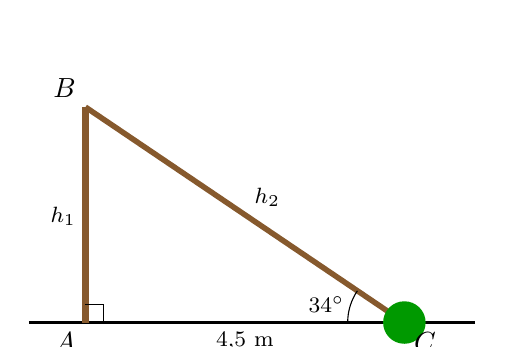
\begin{tikzpicture}[scale=0.9]
  \coordinate (A) at (0,0);
  \coordinate (B) at (0,3.04);
  \coordinate (C) at (4.5,0);
  \draw[thick] (-0.8,0) -- (5.5,0);
  \draw[line width=2.5pt, brown!70!black] (0,0) -- (0,3.04);
  \draw[line width=2pt, brown!70!black] (0,3.04) -- (4.5,0);
  \fill[green!60!black] (4.5,0) circle (0.3);
  \draw (A) ++(0,0.25) -- ++(0.25,0) -- ++(0,-0.25);
  \draw (C) ++(-0.8,0) arc (180:146:0.8);
  \node at (3.4,0.25) {\footnotesize $34^\circ$};
  \node[below] at (2.25,0) {\footnotesize $4{,}5\text{ m}$};
  \node[left] at (0,1.5) {\footnotesize $h_1$};
  \node[above right] at (2.25,1.5) {\footnotesize $h_2$};
  \node[below left] at (A) {$A$};
  \node[above left] at (B) {$B$};
  \node[below right] at (C) {$C$};
\end{tikzpicture}
\end{center}

\vspace{2mm}
\noindent\textbf{Câu 4 (0,5 điểm).}

Giải hệ phương trình sau:\par $\begin{cases} x^3 - 12x = y^3 - 6y^2 + 16 \quad (1) \\ x^2 + 4y^2 + 6xy - 2x - 4y + 9 = 0 \quad (2) \end{cases}$

\vspace{2mm}

\vfill
\begin{center}
  \textbf{--- HẾT ---}
\end{center}
\end{document}
